\documentclass[11pt]{article}
\usepackage[margin=0.72in]{geometry}
\usepackage{graphicx}
\usepackage{hyperref}
\sloppy
\title{N83 radix neural lead probe: local r3}
\author{Exploratory fixed-census analysis}
\date{2026-10-31}
\begin{document}\maketitle
\noindent\textbf{Result.} The model produced no new lead. It flagged 188 of 2,975 censored rows below degree 42; every flag conflicts with its certified lower bound. The fixed prime $m=2$ census retains the same point base and candidate domain. No new factor-base points were generated.
\begin{center}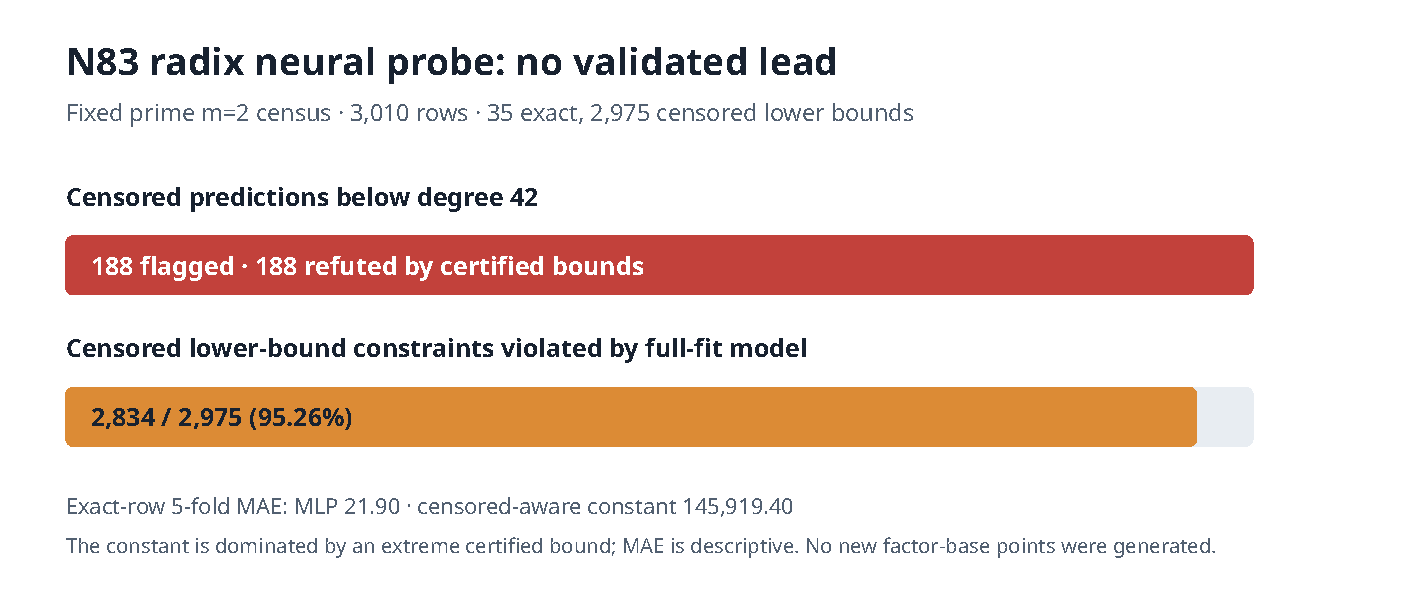
\includegraphics[width=0.98\linewidth]{lead-check.pdf}\end{center}
The five-fold exact-row MAE was 21.9038 for the MLP and 145,919.4019 for the censored-aware constant comparator. The comparator is dominated by the extreme certified lower bound under the fixed grouped objective, so this descriptive MAE comparison does not establish useful model quality. The full-fit network violated 2,834/2,975 (95.26\%) censored lower bounds.

\textbf{Verification.} All 3,010 case files were rehashed against raw census manifest digest recorded in the verification receipt. The nine S3-restored output files matched local hashes. The independent checker reconstructs every prediction (maximum absolute error $2.85\times10^{-14}$), fold assignment, MAE, flag count, contradiction count and lower-bound violation count. See \path{independent-verification.json} and \path{REPORT.md} for full details.

\textbf{Protocol binding.} The run manifest records protocol digest \texttt{66c2eb12...ae4027c4}, matching the v5 file's embedded freeze field. The current committed protocol bytes hash to \texttt{e344d3ec...ba6dac977}, so that recorded digest is not independently confirmed as the file-byte hash. This discrepancy remains explicit in the verification receipt.

\textbf{Run.} ID \path{n83-radix-neural-20261031-local-r3}; local existing Spot host after EKS r1/r2 were cancelled before worker startup. Raw outputs are published under the run-specific S3 prefix documented in REPORT.md. The analysis is scoped to this fixed prime $m=2$ census and does not establish generalization to other curves, $m$, families, or point sets.
\end{document}
